\chapter{Metaheuristics}

In the computer science, the term metaheuristic is accepted for general techniques which are not specific to a particular problem. A metaheuristic is formally defined as an iterative generation process which guides a subordinate heuristic by combining intelligently different concepts for exploring and exploiting the search space \cite{raidl2010metaheuristic}. 

Metaheuristics are strategies that guide the search process to efficiently explore the search space in order to find optimal solutions. Metaheuristic algorithms are approximate and usually non-deterministic and sometimes incorporate mechanisms to avoid getting trapped in confined areas of the search space. There are different ways to classify and describe metaheuristic algorithm \cite{Blum2003}:

\begin{itemize}
\item Nature-inspired vs. non-nature inspired. There are nature-inspired algorithms, like Genetic Algorithms and Ant Algorithms, and non nature-inspired ones such as Tabu Search and Iterated Local Search. 

\item Population-based vs. single point search. Algorithms working on single solutions are called trajectory methods, like Tabu Search, Iterated Local Search and Variable Neighborhood Search. They all share the property of describing a trajectory in the search space during the search process. Population-based metaheuristics perform search processes which describe the evolution of a set of points in the search space.

\item One vs. various neighborhood structures. Most metaheuristic algorithms work on one single neighborhood structure. In other words, the fitness landscape topology does not change in the course of the algorithm. Other metaheuristics, such as Variable Neighborhood Search (VNS), use a set of neighborhood structures which gives the possibility to diversify the search by swapping between different fitness
landscapes.
\end{itemize}

\section{Trajectory Methods}

Trajectory methods are characterized by a trajectory in the search space. Two common trajectory methods are Simulated Annealing and Tabu Search.

\subsection{Simulated Annealing}

Simulated Annealing (SA) is a randomized algorithm that tries to avoid being trapped in local optimum solution by assigning probabilities to deteriorating moves. The SA procedure is inspired from the annealing process of solids. SA is based on a physical
process in metallurgy discipline or solid matter physics. Annealing is the process of obtaining low energy states of a solid in heat treatment \cite{Jaziri2008}. 

The algorithmic framework of SA is described in Alg. \ref{sa}.  The algorithm starts by generating an initial solution in function \textit{GenerateInitialSolution()}. The initial temperature value is determined in function \textit{SetInitialTemperature()} such that the probability for an uphill move is quite high at the start of the algorithm. At each iteration a solution $\mbox{s}_1$ is randomly chosen in function \textit{PickNeighborAtRandom(N(s))}. If \textit{$\mbox{s}_1$} is better than \textit{s}, then \textit{$\mbox{s}_1$} is accepted as new current solution. Else, if the move from \textit{s} to \textit{$\mbox{s}_1$} is an uphill move, \textit{$\mbox{s}_1$}  is accepted with a probability which is a function of a temperature parameter \textit{Tk} and \textit{s} \cite{raidl2010metaheuristic}. 

\begin{algorithm}[h]
  \caption{Simulated Annealing Algorithm}\label{sa}
  \begin{algorithmic}[1]
    
    \State $s\gets GenerateInitialSolution()$
    \State $k\gets 0 $
    \State $Tk\gets SetInitialTemperature()$
    \While{termination conditions not met }
    \State $\mbox{s}_1\gets PickNeighborAtRandom(N (s))$
    \If{$(f(\mbox{s}_1)<f(s))$}
    \State $s\gets\mbox{s}_1$
    \Else $\;$ Accept $\mbox{s}_1$ as new solution with probability p($\mbox{s}_1|$Tk,s) 
    \EndIf
    \State $K\gets K+1$
    \State $Tk\gets AdaptTemperature()$
    \EndWhile
      
  \end{algorithmic}
\end{algorithm}

\subsection{Tabu Search}

Tabu Search (TS) is a metaheuristic that guides a local heuristic search procedure to explore the solution space beyond local optimal and search with short term memory to avoid cycles. Tabu Search uses a  tabu list to keep track of the last  moves, and don’t allow going back to these \cite{Glover1986}.

The basic idea of TS is the explicit use of search history, both to escape
from local minima and to implement a strategy for exploring the search space.
A basic TS algorithm uses short term memory in the form of socalled
tabu lists to escape from local minima and to avoid cycles \cite{Tobergte2013}.

The algorithmic framework of Tabu Search is described in Alg. \ref{tsa}.  The algorithm starts by generating an initial solution in function \textit{GenerateInitialSolution()} and the tabu lists are initialized as empty lists in function \textit{InitializeTabuLists($\mbox{TL}_1$,...,$\mbox{TL}_r$)}. For performing a move, the algorithm first determines those solutions from the neighborhood \textit{N(s)} of the current solution \textit{s} that contain solution features currently to be found in the tabu lists. They are excluded from the neighborhood, resulting in a restricted set of neighbors \textit{$\mbox{N}_a(s)$}. At each iteration the best solution \textit{$\mbox{s}_1$} from \textit{$\mbox{N}_a(s)$} is chosen as the new current solution. Furthermore, in procedure \textit{UpdateTabuLists($\mbox{TL}_1$,...,$\mbox{TL}_r$,s,$\mbox{s}_1$)} the corresponding features of this solution are added to the tabu lists.


\begin{algorithm}[h]
  \caption{Tabu Search Algorithm}\label{tsa}
  \begin{algorithmic}[2]
    
    \State $s\gets GenerateInitialSolution()$
    \State InitializeTabuLists($\mbox{TL}_1$,...,$\mbox{TL}_r$)
    \While{termination conditions not met }
    \State $\mbox{N}_a(s)\gets$ $\{\mbox{s}_1 \in N(s) |\mbox{s}_1$ does not violate a tabu condition, or it satisfies at least one aspiration condition $\}$ 
    \State $\mbox{s}_1\gets argmin\{f(\mbox{s}_2)|\mbox{s}_2 \in \mbox{N}_a(s) \}$
    \State UpdateTabuLists($\mbox{TL}_1$,...,$\mbox{TL}_r$,s,$\mbox{s}_1$)
    \State $s\gets \mbox{s}_1$
    \EndWhile
      
  \end{algorithmic}
\end{algorithm}

\section{Population-based metaheuristics}

Population-based metaheuristics (P-metaheuristics) could be viewed as an iterative improvement in a population of solutions. First, the population is initialized. Then, a new population of solutions is generated. Finally, this new population is integrated into the current one using some selection procedures. The search process is stopped when a stopping criterion is satisfied. Algorithms such as Genetic algorithms (GA), scatter search (SS), estimation of distribution algorithms (EDAs), particle swarm optimization (PSO), bee colony (BC), and artificial immune systems (AISs) belong to this class of metaheuristics \cite{talbi2009metaheuristics}. 

Algorithm \ref{gna} shows the basic structure of GA algorithms. In this algorithm, P denotes the population of individuals. A population of offspring is generated by the application of recombination and mutation operators and the individuals for the next population are selected from the union of the old population and the offspring population \cite{raidl2010metaheuristic}.


\begin{algorithm}[h]
  \caption{Genetic Algorithm}\label{gna}
  \begin{algorithmic}[3]
    
    \State $s\gets GenerateInitialSolution()$
    \State Evaluate(P)
    \While{termination conditions not met }
    \State $\mbox{P}_1\gets$ $Recombine(P)$
    \State $\mbox{P}_2\gets$ $Mutate(\mbox{P}_1)$ 
    \State $Evaluate(\mbox{P}_2)$
    \State $P\gets Select(\mbox{P}_2,P)$
    \EndWhile
      
  \end{algorithmic}
\end{algorithm}

\section{Hybrid  Metaheuristics}

However, in recent years it has become evident that the concentration on a sole metaheuristic is rather restrictive. A skilled combination of a metaheuristic with other optimization techniques, a so called hybrid metaheuristic, can provide a more efficient behavior
and a higher flexibility when dealing with real-world and large-scale problems \cite{Talbi2012}.

A combination of one metaheuristic with components from other metaheuristics is called a hybrid metaheuristic. The concept of hybrid metaheuristics has been commonly accepted only in recent years, even if the idea of combining different metaheuristic strategies and algorithms dates back to the 1980s. Today, we can observe a generalized common agreement on the advantage of combining components from different search techniques and the tendency of designing hybrid techniques is widespread in the fields of operations research and artificial intelligence \cite{raidl2010metaheuristic}. 


There are two main categories of metaheuristic combinations: collaborative combinations and integrative combinations. These are presented in Fig. \ref{fig:metaheuristc} \cite{Raidl2006}.

\begin{figure}[h]
\centering
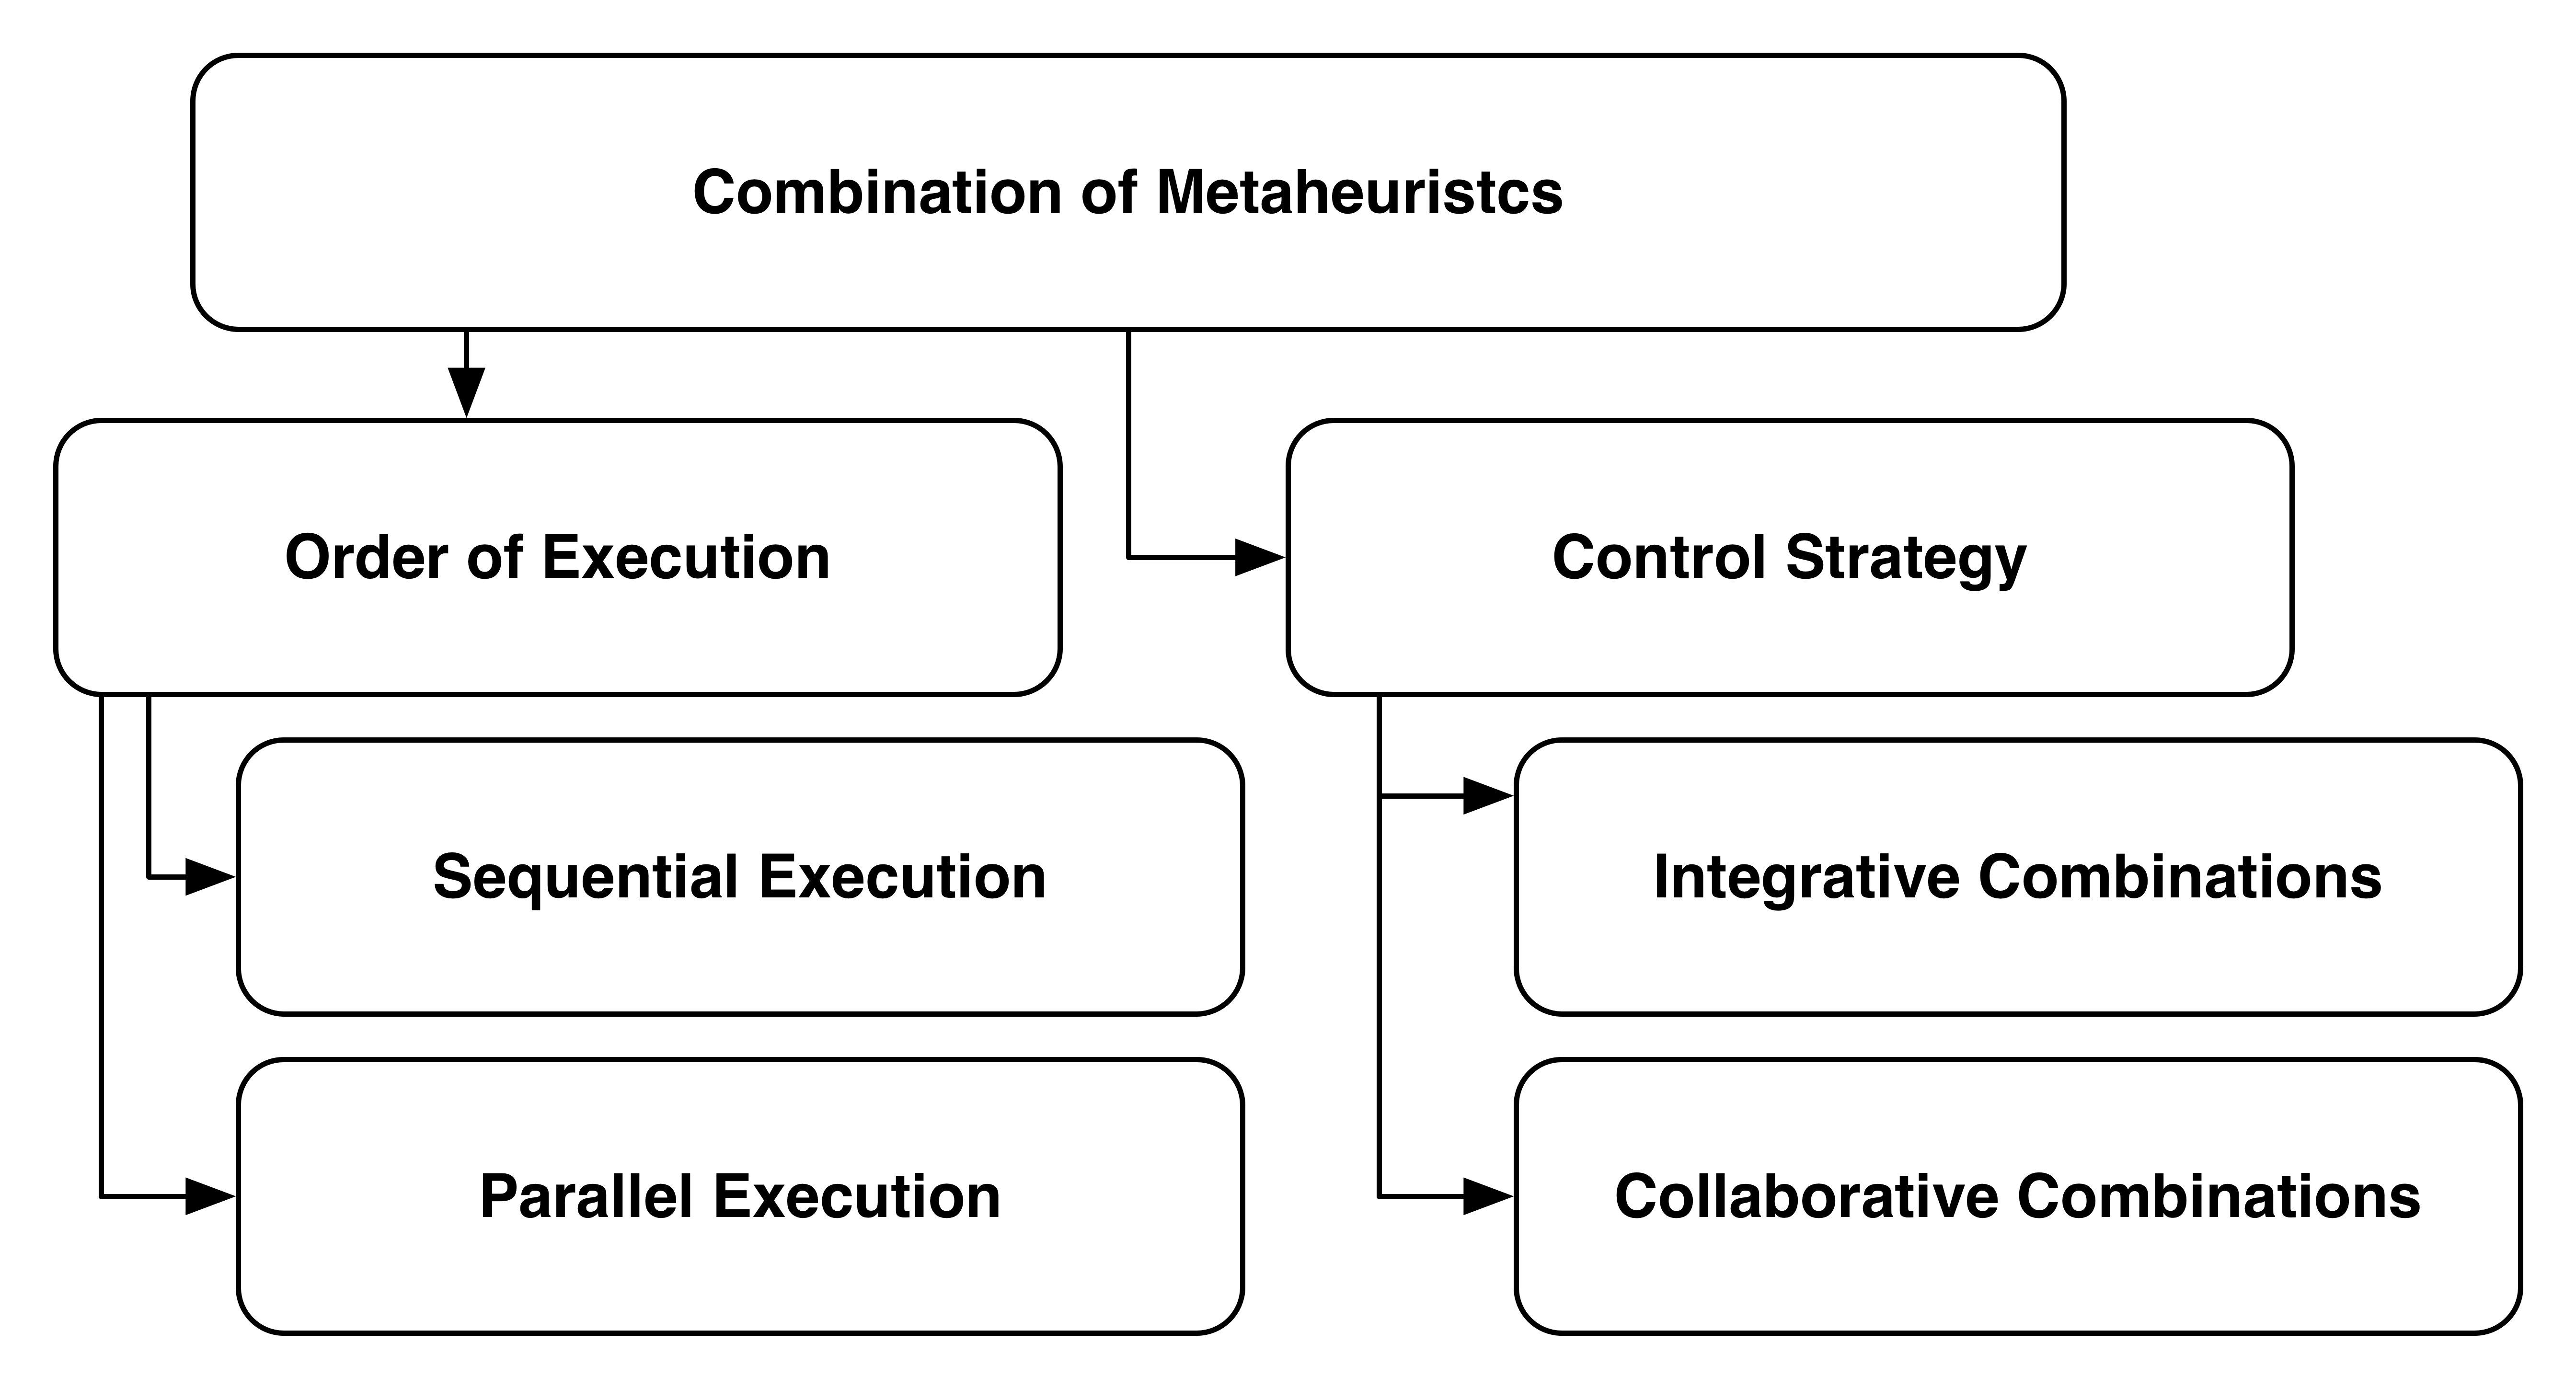
\includegraphics[width=1\textwidth]{./images/metaheuristc2.png}
\caption{Categories of metaheuristc combinations \cite{Puchinger2005} }
\label{fig:metaheuristc}
\end{figure}

Collaborative combinations use an approach where the algorithms exchange information, but are not part of each other. In this approach, algorithms may be executed sequentially or in parallel. 

One of the most popular ways of metaheuristic hybridization consists in the use of trajectory methods inside population-based methods. Population-based methods are better in identifying promising areas in the search space from which trajectory methods can quickly reach good local optima. Therefore, metaheuristic hybrids that can effectively combine the strengths of both population-based methods and trajectory methods are often very successful \cite{raidl2010metaheuristic}.


The work uses a type of collaborative combination with sequential execution with two trajectory methods (Tabu Search and Simulated Annealing) and Genetic Algorithms.


